\documentclass{beamer}

\usepackage{graphicx,hyperref,udesc,url}
\usepackage[utf8]{inputenc}
\usepackage[T1]{fontenc}
\usepackage{booktabs}
\usepackage[portuges]{babel}

\usepackage{pgf,tikz}
\usepackage{tkz-graph}
\usetikzlibrary{shapes.geometric}


\title[SDN]{Software Defined Network, Openflow e Mininet}

\author[Renan, Ruan, Ricardo]{
    Renan S. Silva, Ruan P. Medeiros, Ricardo Sohn\\\medskip
    {\small \url{uber.renan@gmail.com}} \\ 
    {\small \url{pm.ruan@gmail.com}}\\
    {\small \url{ricardosohn@gmail.com}}
}

\institute[UDESC]{
    Departamento de Ci\^encia da Computa\c{c}\~ao \\
    Centro de Ci\^encias e Tecnol\'ogias\\
Universidade do Estado de Santa Catarina}

\begin{document}

\begin{frame}
    \titlepage
\end{frame}

\begin{frame}
    \frametitle{Sum\'ario}
    \tableofcontents
\end{frame}

\section{Objetivo}

\begin{frame}
    \frametitle{Objetivo}
    Analisar o desempenho do Mininet em relação a redes tradicionais na transmissão de fluxos de dados de tamanho médio.
\end{frame}

\begin{frame}
    \frametitle{Motivação}
    \begin{itemize}
        \item A \textit{Software Defined Network} (SDN) é um novo paradigma de rede que permite um nível de controle e flexibilidade inédito da rede.
        \item O Hardware é caro.
        \item É necessário alternativas viáveis para impulsionar o desenvolvimento cientifico.
    \end{itemize}
\end{frame}

\section{Software Defined Network}

\begin{frame}
    \frametitle{Software Defined Network}

    \begin{center}
        {\huge Software Defined Network}
    \end{center}
\end{frame}

\begin{frame}
    \frametitle{Software Defined Network}

    Redes tradicionais

    \begin{itemize}
        \item Redes tradicionais são complexas e dificeis de gerenciar.

        \begin{itemize}
            \item É necessário usar recursos de baixo nível.
            \item Muitas vezes específicos do fabricante.
            \item Reconfiguração autmatica e mecanismos de resposta não se mostram suficiente.
        \end{itemize}
        \item São verticalmente integradas. \textit{Data plane} e \textit{Control plane} estão juntas no mesmo dipositivo.
    \end{itemize}
\end{frame}


\begin{frame}
    \frametitle{Software Defined Network}

    O que é

    \begin{itemize}
        \item A \textit{Open Networking Foundation} define SDN como sendo a separação lógica do \textit{Data Plane} e \textit{Control Plane}.
        \item \textit{Switchs} são simples redirecionadores de tráfego.
        \item Controle da rede é logicamente centralizado.
        \item Regras são definidas baseadas em fluxo, não em destinos.
    \end{itemize}
\end{frame}

\begin{frame}
    \frametitle{\textit{Data plane}}

    No SDN, o \textit{Data plane} é o elemento da rede que guiado por uma entidade controladora é reponsável por:

    \begin{itemize}
        \item Inspecionar
        \item Modificar
        \item \textit{Dropping}
        \item \textit{Forwarding}
    \end{itemize}

\end{frame}

\begin{frame}
    \frametitle{\textit{Data plane}}

    O \textit{Data plane}, guiado pelo controlador, pode desempenhar varios papeis da rede:

    \begin{itemize}
        \item \textit{Switch}
        \item Roteador
        \item \textit{Firewall}
        \item \textit{Load Balancer}
        \item \textit{Traffic shaper}
    \end{itemize}

\end{frame}

\begin{frame}
    \frametitle{\textit{Control plane}}

    O \textit{Control plane} é responsável por controlar e monitorar o \textit{Data plane}.

    \begin{itemize}
        \item Define como um dispositivo se comporta na rede.
        \item O \textit{Control plane} executa um \textit{Network Operating System} (NOS).
        \item Se comunica com o \textit{Data plane} atravéz da \textit{Southbound API}.
        \item Se comunica com o mundo externo atravéz da \textit{Northbound API}.
    \end{itemize}
\end{frame}

\begin{frame}
    \frametitle{Visão Geral}

    \begin{figure}
        \centering
        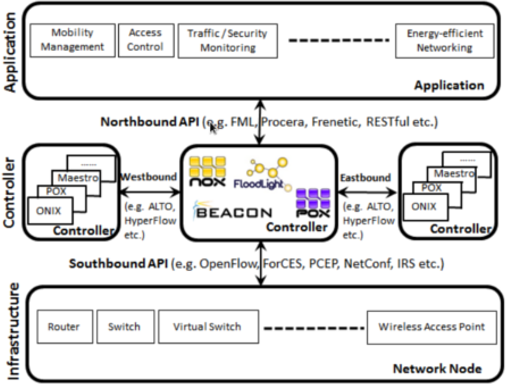
\includegraphics[width=0.75\linewidth]{sdnARCH}
        \label{hue}
        \caption{Visão Geral}
    \end{figure}

\end{frame}

%\section{\textit{OpenFlow}}
\section{OpenFlow}

\begin{frame}
    \frametitle{OpenFlow}

    \begin{center}
        {\huge{OpenFlow}}
    \end{center}

\end{frame}

\begin{frame}
    \frametitle{OpenFlow}

    O \textit{Openflow} é uma das diversas \textit{Southbound API}s disponíveis.

    \begin{itemize}
        \item Mantida e desenvolvida pela ONF.
        \item \textit{Open source}.
        \item Padronizada.
        \item Suportada por diversos fabricantes.
        \item Operação reativa ou pró-ativa
    \end{itemize}
\end{frame}

\section{Mininet}

\begin{frame}
    \frametitle{Miniet}

    \begin{center}
        {\huge Mininet}
    \end{center}

\end{frame}

\begin{frame}
    \frametitle{Mininet}

    O Mininet é um simulador de redes.

    \begin{itemize}
        \item Utiliza \textit{Linux Container Architecture} e \textit{Network Namespaces}.
        \begin{itemize}
            \item Provê isolamento do sistema hospedeiro.
            \item Permite a ligação com uma rede real.
            \item É executado dentro de uma \textit{Jail}.
        \end{itemize}
        \item Licença baseada na licença BSD.
        \item Criado para impulsionar o desenvolvimento e uso do SDN/OpenFlow.
        \item Utilizado atravéz de sua API Python ou de um Shell interativo.
    \end{itemize}
\end{frame}

\begin{frame}
    \frametitle{Mininet}

    \begin{itemize}
        \item Por rodar em cima do kernel Linux é possível desenvolver aplicativos que são testados no Mininet
            e implantados em uma rede real com pouca ou nenhuma alteração.
        \item Permite o desenvolvimento de protótipos e experimentos em um ambiente autocontido que pode ser
            distruido e reproduzido com facilidade.
        \item Uma máquina virtual modelo está disponível em \url{http://mininet.org/download/}.
    \end{itemize}
\end{frame}


\begin{frame}
    \frametitle{Limitações}

    Algumas limitações do Mininet

    \begin{itemize}
        \item Sistemas de arquivos compartilhado.
        \begin{itemize}
            \item Economiza espaço, simplifica compartilhamento de arquivos entre \textit{hosts}.
            \item Pode criar conflitos com programas/\textit{daemons} que necessitem de configurações diferentes.
        \end{itemize}
        \item \textit{Hosts} virtuais competem por tempo de CPU.
        \item Os \textit{hosts} possuem o mesmo PID.
        \item Limitado as sistemas GNU/Linux.
    \end{itemize}
\end{frame}

\section{Experimentos}

\begin{frame}
    \frametitle{Experimentos}

    \begin{center}
        {\huge Experimentos}
    \end{center}

\end{frame}

\begin{frame}
    \frametitle{Benchmark da Rede}

    Cópia de arquivos de $256$, $512$, $768$ e $1024$ Megabytes.

    \begin{itemize}
        \item Cópia realizada via \textit{rsync}
        \item \textit{rsync} tunelado via \textit{ssh} para realizar a transferência via rede.
        \item Arquivos de conteúdo aleatório gerados com via \textit{/dev/urandom}.
        \item Cache limpo antes de cada teste para melhorar a reprodutibilidade do experimento.
    \end{itemize}
\end{frame}

\begin{frame}
    \frametitle{Ambiente de testes}

    Foram utilizados 3 ambientes de testes:

    \begin{itemize}
        \item Mininet executando na máquina virtual disponibilizada pelo desenvolvedor.
        \item Núvem baseada em OpenStack (F$109$).
        \item Rede física (F$112$).
    \end{itemize}
\end{frame}

\begin{frame}
    \frametitle{Topologia de rede utilizada}

    \begin{figure}[h]
        \centering
        \begin{tikzpicture}
            \node[text centered] at (4,2) (s1) {$S1$};

            \node[text centered] at (2,0) (h1) {$H1$};
            \node[text centered] at (6,0) (h2) {$H2$};

            \draw[-, line width = 1] (s1) -- node[above,font=\footnotesize]{$ $} (h1);
            \draw[-, line width = 1] (s1) -- node[above,font=\footnotesize]{$ $} (h2);
            \label{fig_topo}
        \end{tikzpicture}
        \caption{Topologia da rede do ambiente de testes}
    \end{figure}
\end{frame}

\begin{frame}
    \frametitle{Resultados}

    \begin{center}
        {\huge Resultados}
    \end{center}
\end{frame}

\begin{frame}
    \frametitle{Resultados do Mininet}

    \begin{figure}[ht]
        \centering
        \begin{minipage}[b]{0.49\linewidth}
            \centering
    %
            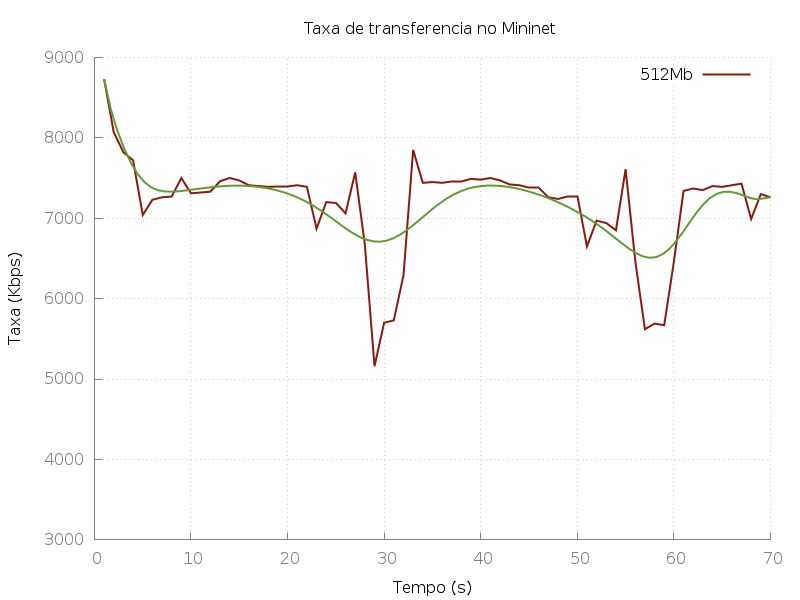
\includegraphics[width=\textwidth]{data/data_cp_mininet/taxa_512}
    %
            \caption{Taxa de transferência de arquivo de 512 Megabytes no Mininet}
            \label{fig:mininet512}
        \end{minipage}
    %
        \begin{minipage}[b]{0.49\linewidth}
            \centering
    %
            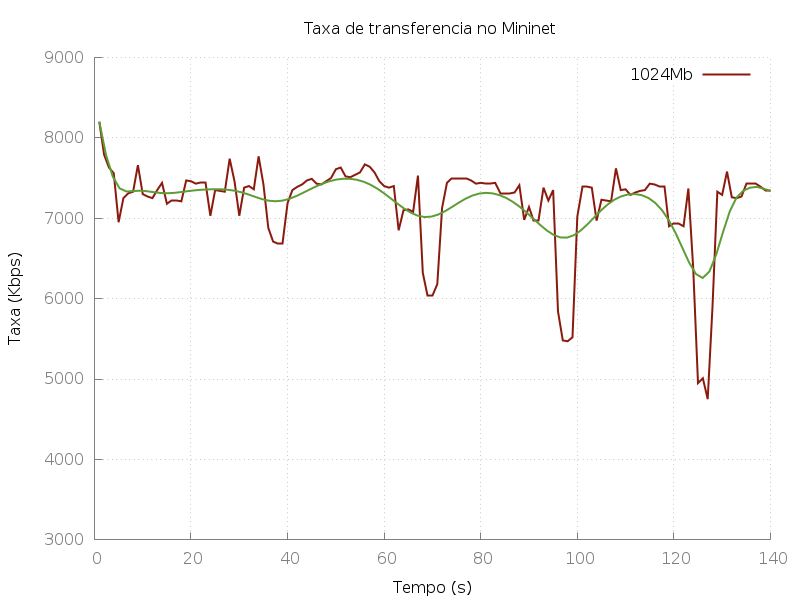
\includegraphics[width=\textwidth]{data/data_cp_mininet/taxa_1024}
    %
            \caption{Taxa de transferência de arquivo de 1024 Megabytes no Mininet}
            \label{fig:mininet1024}
        \end{minipage}
    \end{figure}
    \end{frame}

\begin{frame}
    \frametitle{Resultados do OpenStack}

    \begin{figure}[ht]
        \centering
        \begin{minipage}[b]{0.49\linewidth}
            \centering
    %
            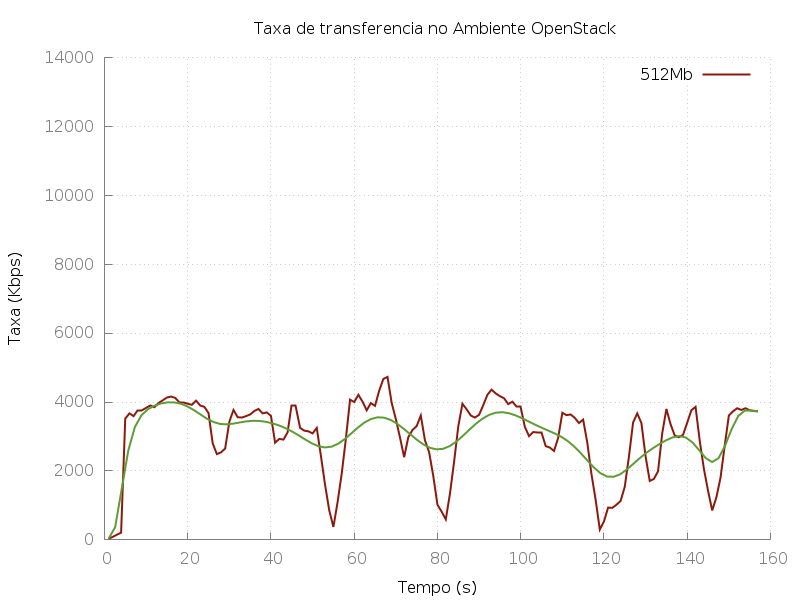
\includegraphics[width=\textwidth]{data/data_cp_openstack/taxa_512}
    %
            \caption{Taxa de transferência de arquivo de 512 Megabytes no OpenStack}
            \label{fig:openstack512}
        \end{minipage}
    %
        \begin{minipage}[b]{0.49\linewidth}
            \centering
    %
            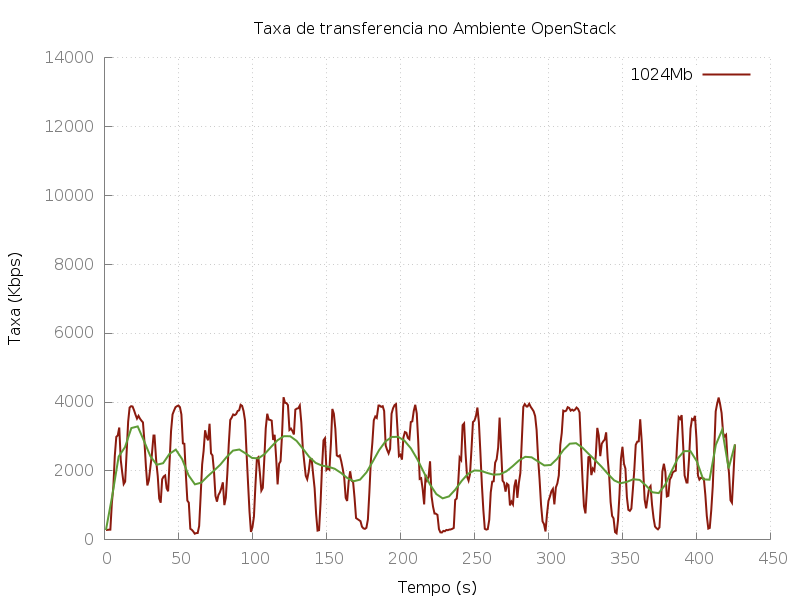
\includegraphics[width=\textwidth]{data/data_cp_openstack/taxa_1024}
    %
            \caption{Taxa de transferência de arquivo de 1024 Megabytes no OpenStack}
            \label{fig:openstack1024}
        \end{minipage}
    \end{figure}
\end{frame}

\begin{frame}
    \frametitle{Resultados da rede física}

    \begin{figure}[ht]
        \centering
        \begin{minipage}[b]{0.49\linewidth}
            \centering
    %
            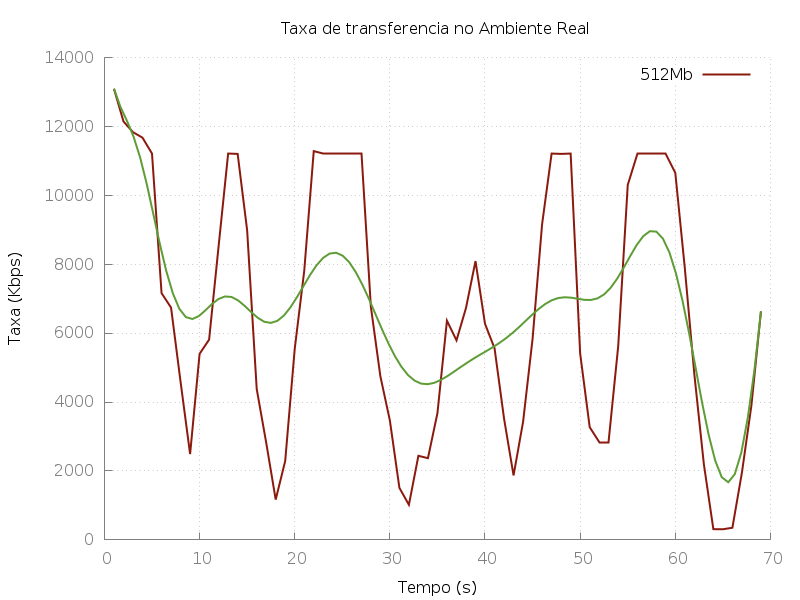
\includegraphics[width=\textwidth]{data/data_cp_real/taxa_512}
    %
            \caption{Taxa de transferência de arquivo de 512 Megabytes no ambiente físico}
            \label{fig:real512}
        \end{minipage}
    %
        \begin{minipage}[b]{0.49\linewidth}
            \centering
    %
            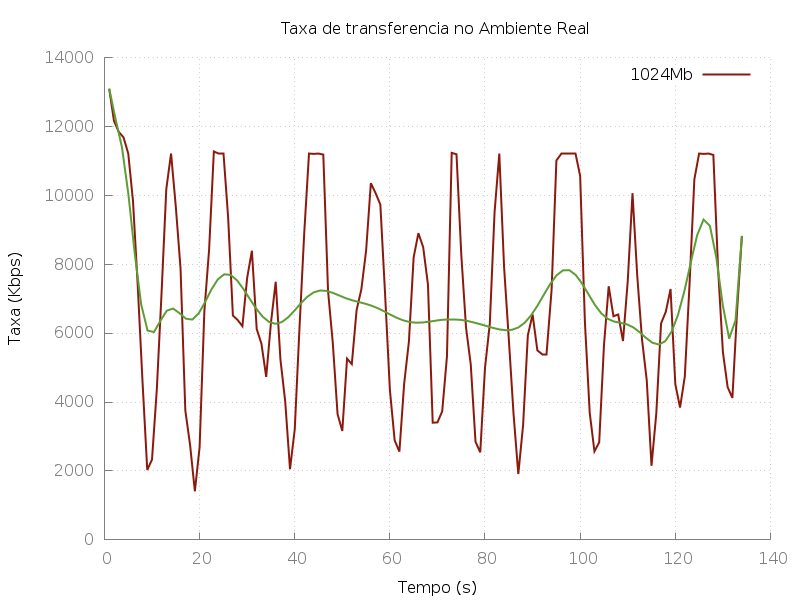
\includegraphics[width=\textwidth]{data/data_cp_real/taxa_1024}
    %
            \caption{Taxa de transferência de arquivo de 1024 Megabytes no ambiente físico}
            \label{fig:real1024}
        \end{minipage}
    \end{figure}
\end{frame}

\begin{frame}
    \frametitle{Comportamento anormal}

    \begin{figure}[h]
        \centering
        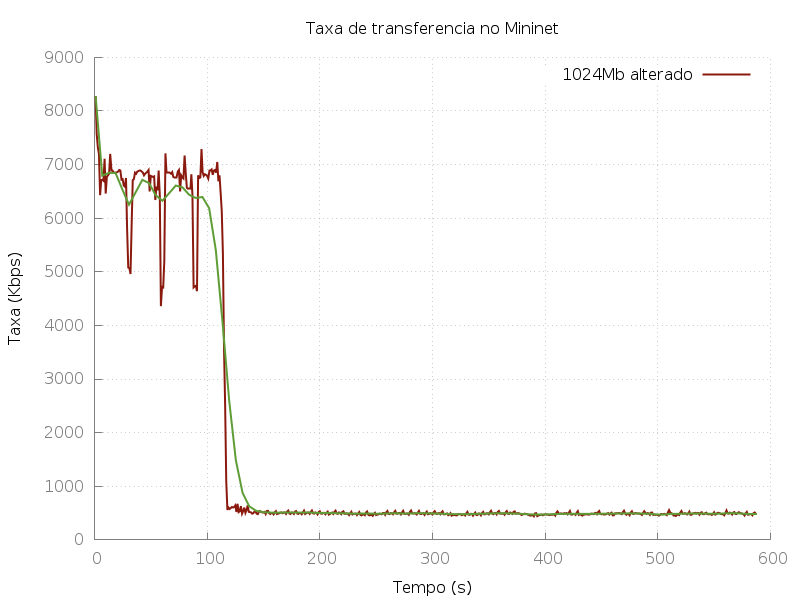
\includegraphics[width=.65\textwidth]{data/data_cp_mininet/taxa_1024_hue}
        \caption{Comportamento anormal no Mininet}
        \label{fig:zoera}
    \end{figure}
\end{frame}

\begin{frame}
    \frametitle{Análise}

    \begin{center}
        {\huge Análise}
    \end{center}
\end{frame}

\begin{frame}
    \frametitle{Transferência média}

    Taxa de transferência média observada

    \begin{table}[h]
        \centering
        \begin{tabular}{|l|l|l|l|}
            \hline
            Tamanho do arquivo & Real         &  Mininet      &  OpenStack   \\ \hline
            256  Megabytes     & $6.17$ MB/s  &  $6.67$ MB/s  &  $2.57$ MB/s \\
            512  Megabytes     & $6.07$ MB/s  &  $7.15$ MB/s  &  $2.26$ MB/s \\
            768  Megabytes     & $7.62$ MB/s  &  $6.61$ MB/s  &  $2.36$ MB/s \\
            1024 Megabytes     & $6.64$ MB/s  &  $7.17$ MB/s  &  $2.10$ MB/s \\ \hline
        \end{tabular}
        \caption{Taxa de transferência média}
        \label{tab_taxa_media}
    \end{table}

\end{frame}

\begin{frame}
    \frametitle{Desvio padrão}

    Desvio padrão das taxas observadas

    \begin{table}[h]
        \centering
        \begin{tabular}{|l|l|l|}
            \hline
            Tamanho do arquivo & Real         &  Mininet    \\ \hline
            256  Megabytes     & $4.26$       &  $0.560$    \\
            512  Megabytes     & $3.76$       &  $0.594$    \\
            768  Megabytes     & $2.47$       &  $0.645$    \\
            1024 Megabytes     & $2.95$       &  $0.549$    \\ \hline
        \end{tabular}
        \caption{Desvio padrão da taxa de transferência}
        \label{tab_taxa_desvio}
    \end{table}
\end{frame}

\begin{frame}
    \frametitle{Resultados da rede física}

    \begin{figure}[ht]
        \centering
        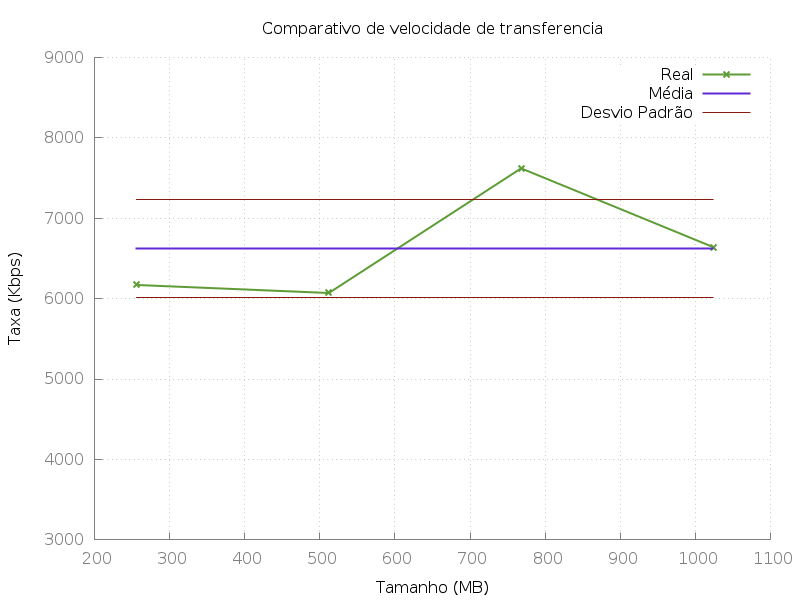
\includegraphics[width=0.65\textwidth]{data/taxa_real}
        \caption{Taxa, média e desvio padrão de transferência no ambiente real}
        \label{fig:taxa_mininet}
    \end{figure}
\end{frame}

\begin{frame}
    \frametitle{Resultados do Mininet}

    \begin{figure}[ht]
        \centering
        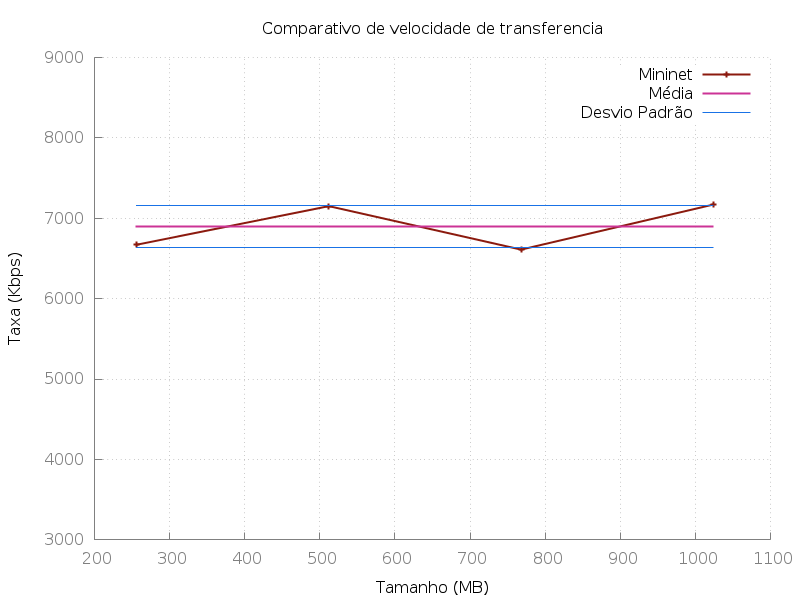
\includegraphics[width=0.65\textwidth]{data/taxa_mininet}
        \caption{Taxa, média e desvio padrão de transferência no ambiente Mininet}
        \label{fig:taxa_mininet}
    \end{figure}
\end{frame}

\begin{frame}
    \frametitle{Anomalia}

    Comportamento anomal no Mininet

    \begin{itemize}
        \item Queda de 6.9 MB/s para 495 KB/s.
        \item Variação de apenas 26.6 BK/s após a queda.
        \item Aconteceu várias vezes.
        \item Nenhuma vez voltou a velocidade padrão.
        \item Resultados com anomalias foram descartados.
    \end{itemize}
\end{frame}

\section{Conclusão}

\begin{frame}
    \frametitle{Conlusão}

    \begin{center}
        {\huge Conclusão}
    \end{center}

\end{frame}

\begin{frame} \frametitle{Conlusão}

    Conclusão

    \begin{itemize}
        \item Mininet apresentou comportamentos anormais.
        \item Mininet se mostrou uma ferramenta simples de se usar e bem documentada.
        \item Desempenho do Mininet se mostrou levemente superior, $4.45\%$.
        \item Rede física apresentou grande variação enquanto que o Mininet se manteve estável, apenas $17\%$ da variação da rede física.
        \item Resultados com anomalias nos ambientes Mininet e OpenStack foram descartados.
        \item Possível interferência externa em ambos os casos.
        \begin{itemize}
            \item Não foi possível isolar o problema.
        \end{itemize}
    \end{itemize}
\end{frame}

\begin{frame}
    \frametitle{Alternativas}

    Alternativas ao Mininet

    \begin{itemize}
        \item \textbf{Maxinet} Tem como objetivo rodar o Mininet de forma distribuida com a finalidade de simular
            redes maiores do que o Mininet permite, sem afetar a fidelidade do desempenho.

        \item \textbf{Mininet-Hifi} Tem como objetivo aumentar a fidelidade e reprodutibilidade dos experimentos
            realizados no Mininet.
    \end{itemize}
\end{frame}

\begin{frame}
    \frametitle{Trabalhos futuros}

    Trabalhos futuros

    \begin{itemize}
        \item Executar os testes novamente em outro ambiente, versões mais novas/velhas dos pacotes.
        \item Experiementar em outras alternativas ao Mininet.
    \end{itemize}
\end{frame}

\begin{frame}
    \frametitle{Perguntas}

    \begin{center}
        {\huge Perguntas?}
    \end{center}
\end{frame}

\nocite{archoverview}
\nocite{archteture}
\nocite{newnorm}
\nocite{management}
\nocite{onf:cpe}
\nocite{survey}
\nocite{networkinalaptop}
\nocite{mininetproto}
\nocite{maxinet}
\nocite{mininethifi}

\section{Refer\^encias}
\begin{frame}[allowframebreaks]
    \frametitle{Refer\^encias}
    \bibliographystyle{abnt-alf}
    \bibliography{bibliografia}
\end{frame}


\end{document}
